\newpage


\section{Convolutional Neural Networks (CNNs)}
\label{sec:convolutional-neural-networks-(cnns)}

Convolutional Neural Networks introduce a powerful tool that fits very well when working in the context of image elaboration.
This tool, which gives the name to the networks, is the \textbf{convolution layer}.

\paragraph{Convolution}
It applies the homonymous mathematical operation by combining two functions to produce a third one, in the discrete case:
\[(f\ast g)(n) = \sum f(m)g(n-m)\]
Where, in the context of images, $f$ could represent an image and $g$ a kernel.

More intuitively the kernel combines the pixels of an image in a window altered them values based on the neighborhood.
In neural network this is not any different as the weighted inputs are convoluted by the kernel specification.

In image processing convolution is a basic step for many tasks, and it becomes powerful in neural networks
as the model learns the kernel matrices during the training process.
The power in applying convolutions to the data is that it alters its information to better show features of
the image; i.e.\ from simple lines in the beginning of the network to complex shapes in deeper convolutions.

In keras this is obtained by the \textbf{Conv2D}\cite{con2d} layer object, such as:
\begin{verbatim}
x = keras.layers.Conv2D(
    filters=64, kernel_size=(3,3), padding="same", activation="relu"
)
\end{verbatim}

\paragraph{Pooling}
In order to reduce the amount of parameters and improve generalization one can use the \textbf{Pooling} layer.
The pooling operation simply down-samples the feature map of the data. In \textit{keras} this is achieved by any implementation
of the pooling operation. As empirical performance between the various methods\cite{bieder2021comparison}
doesn't favor any precise method, the \textbf{MaxPooling2D}\cite{maxpooling2d} was used.

\\

\paragraph{}
For a long time CNNs have been the state of the art for various fields involving machine learning, including Computer Vision.
Now that transformers have become popular CNNs might have been outclassed, but the question is still open for debate.\cite{wang2023cnns}
Besides being very effective the fact that they are both easier to train and less memory constraining were other good reasons
to favor CNNs instead of the simple MLPs approach.

\subsection{Model Structure}
% todo finish with images

\paragraph{First Model}
For the first model, shown in Figure \ref{fig:custom_cnn}, each convolution layer, two in total, is followed by pooling one.
A good rule when designing CNN, confirmed by empirical evidence i.e. on \textit{VGG-16} \ref{subsubsec:vgg16},
is to increase the number of filters in deeper layers as the down-sampling reduces the power of representation of the network.
This rule was applied to the definition of the model.

\paragraph{}
In its first definition no image augmentation procedure was used.
The model was overfitting the training set with $acc=88\%$ and $l = 0.6591$.

We redefined the model using augmentation (\ref{subsec:data-augmentation}). This resulted in a similar model
in terms of accuracy but a noticeable decrease in loss meaning the model is more certain about more classifications.
The k-fold-CV estimates, after learning the optimal learning parameters,  reported in \ref{tab:kfoldcnn} are coherent with the final measured model performance being:
$acc=89.36\%$ and $l_{0-1} = 0.1014$. % todo qui valori veri non falsi

\begin{figure}[h]
    \centering
    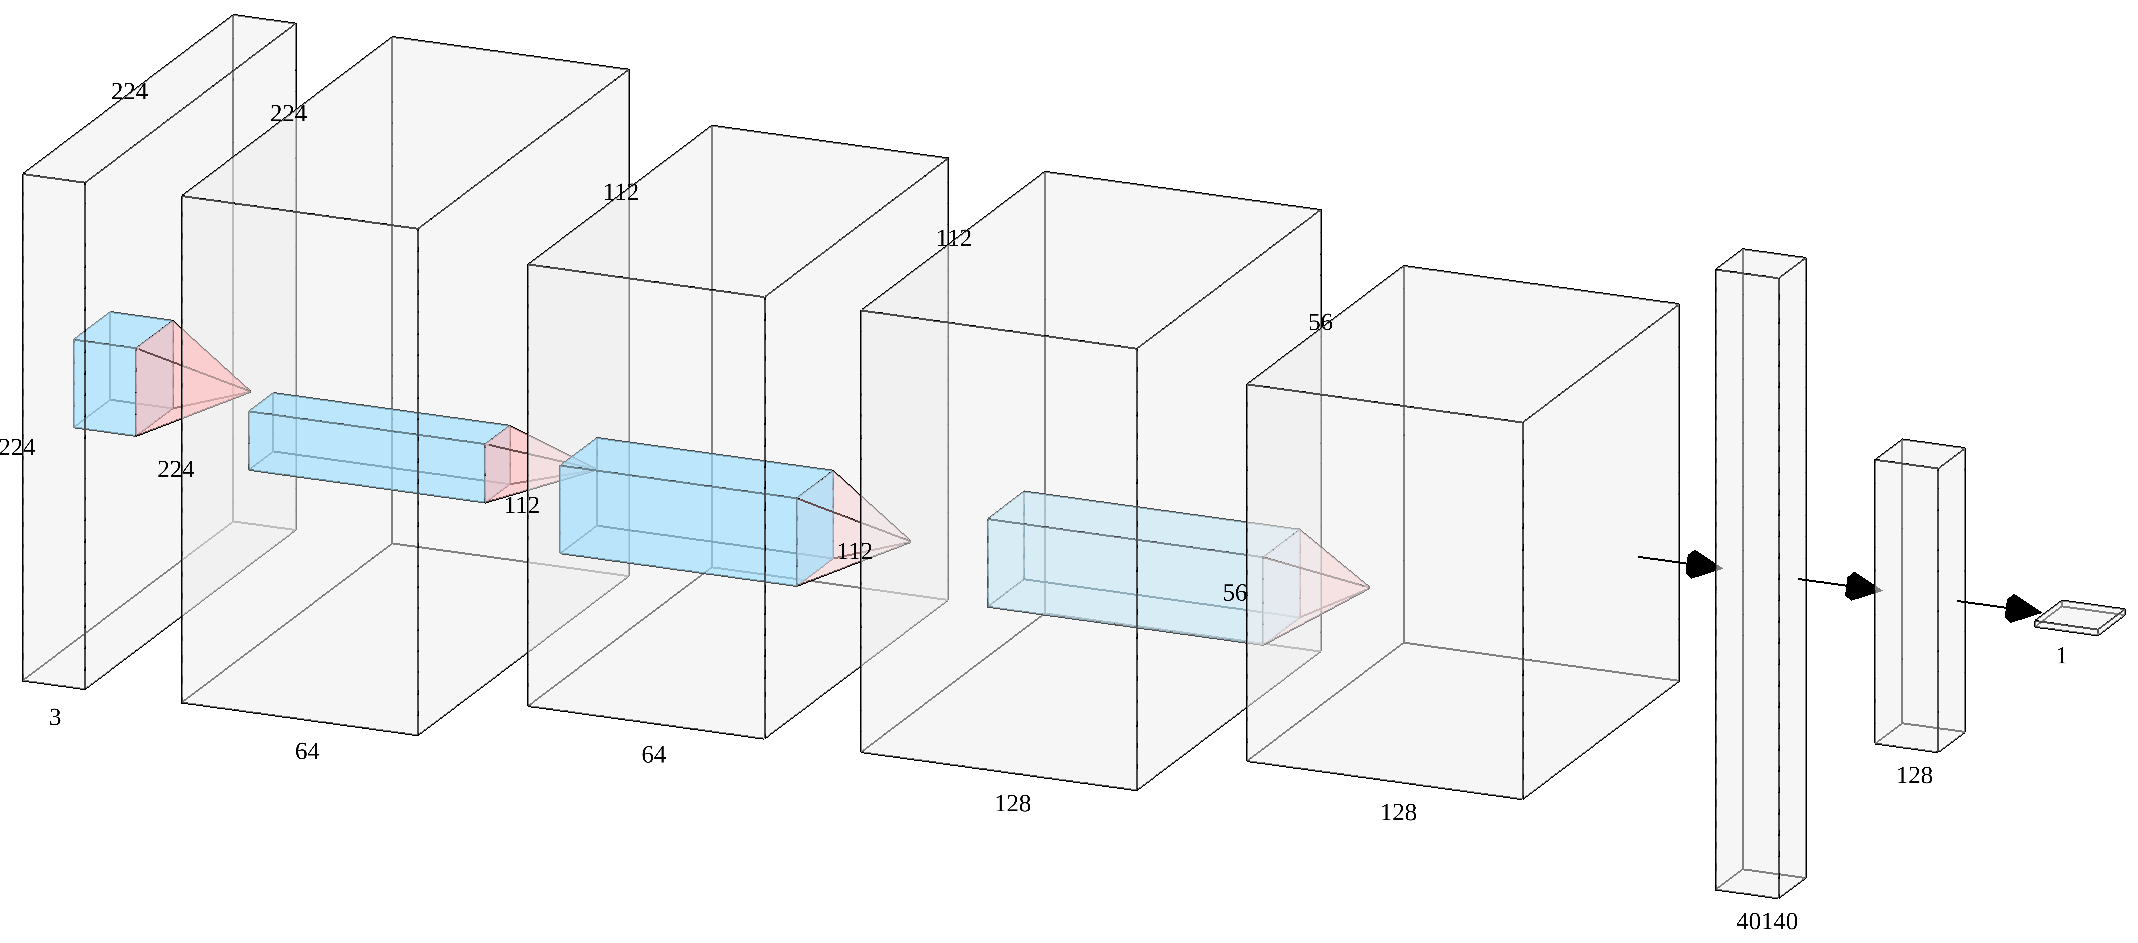
\includegraphics[scale=0.15]{imgs/custom-cnn-one}
    \caption{
        Graphical representation of the first CNN model.\\
        \textit{Image generated via the NN-SVG tool}
    }\label{fig:custom_cnn}
\end{figure}

\paragraph{Second Model}

To reduce overfitting on the first model we tried defining a model with fewer parameters.
The structure of the model is defined in Figure \ref{fig:second-conv-net-structure}
and has, only on the first Convolution layer, a wider kernel of size $(5\times5)$ in the hope of the network to capture a broader context.

For this network the learning parameters have not been trained but the optimal configuration for the first conv network
was used instead.
The risk estimates for the network performance are reported in the Table \ref{tab:kfoldcnn}.

The final model is in line with the expected performance as it measured $acc=89.70\%$ and $l_{0-1}=0.1030$ on the test set.
If we tuned the training hyperparameters specifically for this architecture we might have gotten a better model.


\begin{figure}
    \centering
    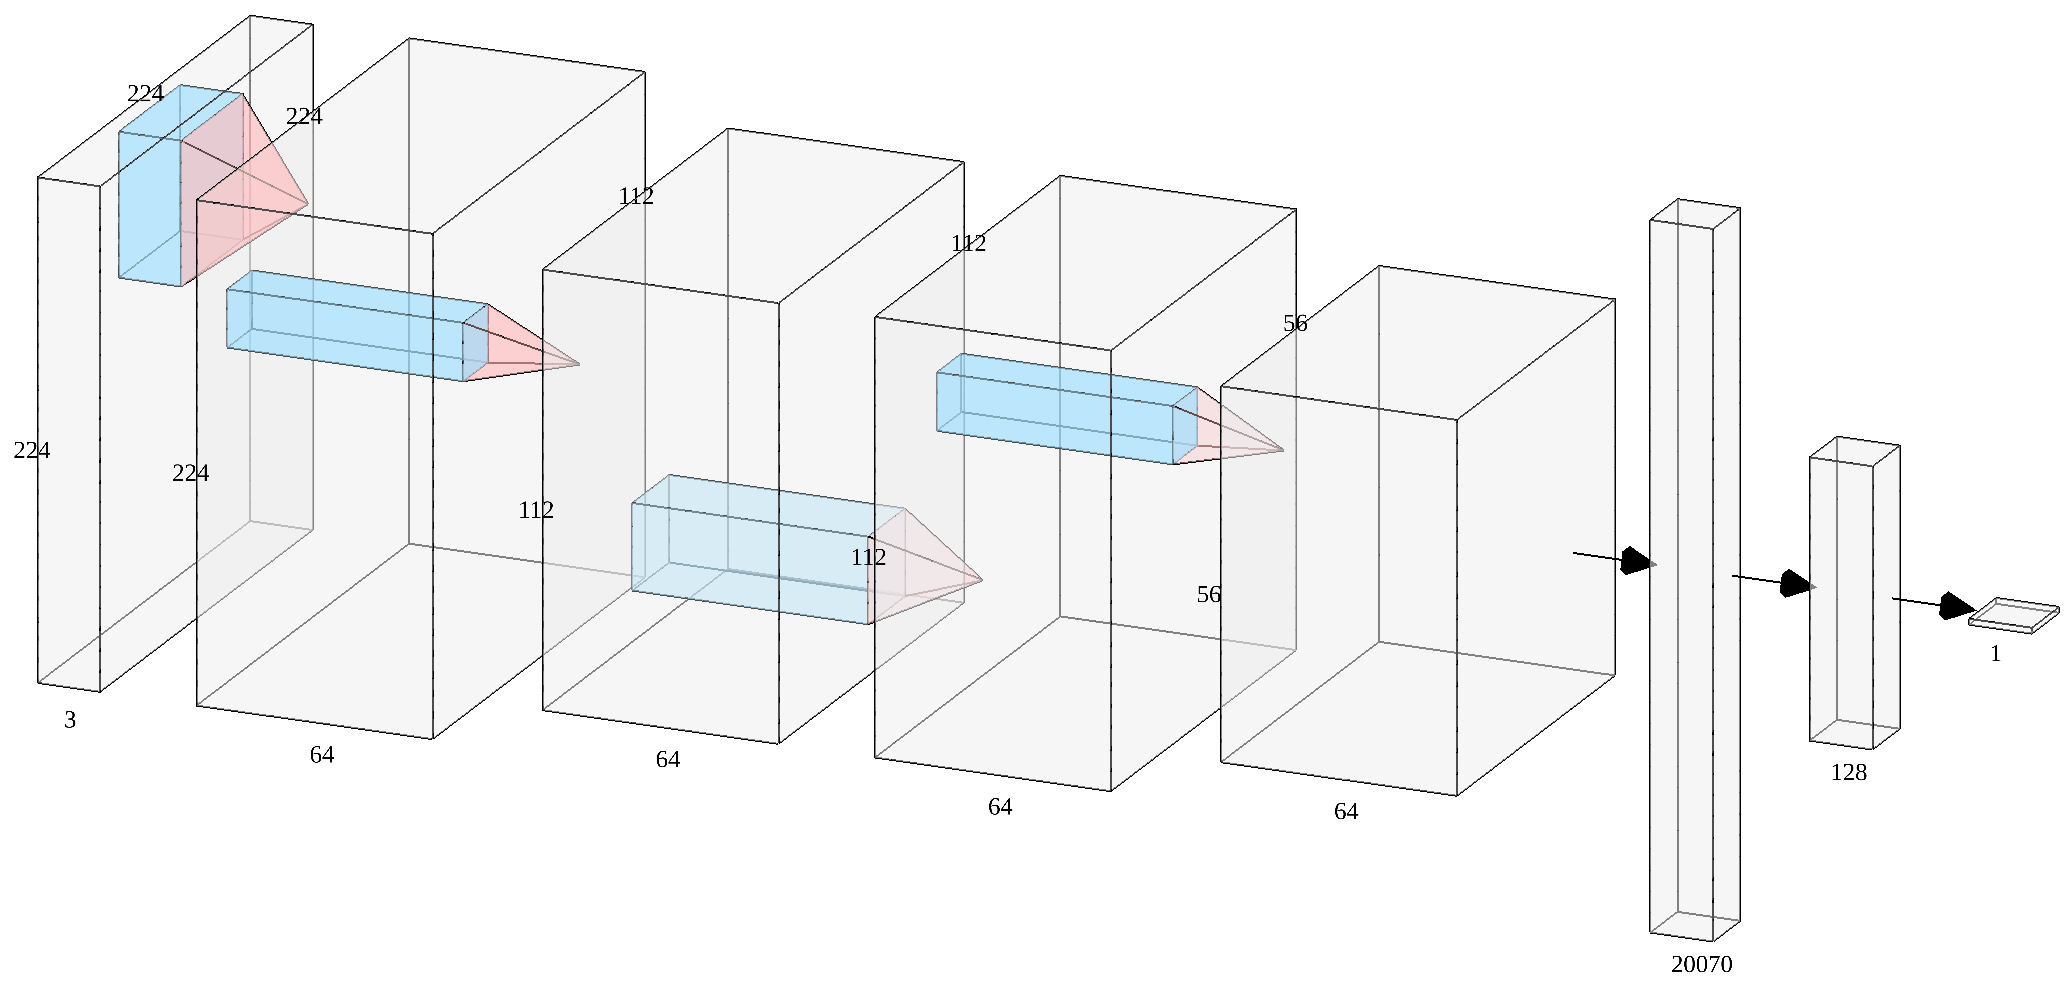
\includegraphics[scale=0.15]{/home/jacopo/PycharmProjects/muffin-stat-project/report/imgs/second-conv-net-structure}
    \caption{
        Graphical representation of the second CNN model.\\
        \textit{Image generated via the NN-SVG tool}
    }
    \label{fig:second-conv-net-structure}
\end{figure}


\begin{table}
    \centering
    \begin{tabular}{ | c | c | c | }
        \hline
        $k$ & $accuracy$ & $l_{0-1}$ \\
        \hline\hline
        0   & 0.8666     & 0.1334    \\
        \hline
        1   & 0.9029     & 0.0971    \\
        \hline
        2   & 0.8707     & 0.1293    \\
        \hline
        3   & 0.8935     & 0.1065    \\
        \hline
        4   & 0.8808     & 0.1192    \\
        \hline
        \hline
        avg & 0.8829     & 0.1171    \\
        \hline
    \end{tabular}
    \quad
    \begin{tabular}{| c | c | c |}
        \hline
        $k$ & $accuracy$ & $l_{0-1}$ \\
        \hline\hline
        0   & 0.8910     & 0.1090    \\
        \hline
        1   & 0.8970     & 0.1030    \\
        \hline
        2   & 0.8377     & 0.1623    \\
        \hline
        3   & 0.8986     & 0.1014    \\
        \hline
        4   & 0.8986     & 0.1014    \\
        \hline
        \hline
        avg & 0.8846     & 0.1154    \\
        \hline
    \end{tabular}
    \caption{
        Left the first model's \textit{k-fold-CV} estimates, right the second one's.
    }

    \label{tab:kfoldcnn}
\end{table}

\subsubsection{Autotuned CNN}
\label{subsubsec:autotuned}
The presented CNNs yield discrete results which might be for their simplicity so a better and more
complex structure should be identifiable in some way.
Instead of going on by process of trial and error we try to learn the architecture.

In order to do achieve this result while still testing a good amount of combinations, the search space
was confined to the following variables:
\begin{description}
    \item [convolutional\_layers] The amount of $(CONV \rightarrow POOL)$ layers to build.\\
    For each of these, the pooling layer parameters were fixed.
    \item[filters\_i] Number of filters, a power of two from 16 to 256.\\
    The setting is referred to the specific convolution layer $i$
    \item[kernel\_i] The square size of the kernel chosen from the set of values: $\{3,5\}$.
    The setting is referred to the specific convolution layer $i$
    \item[hidden\_layers] Number of dense layers that follow the convolutional ones
    \item[units\_i] Number of units for the dense layer $i$
\end{description}

The optimization process has run for a total of 40 iterations and resulted in various models with a close performance.
From the results a trend indicates that networks with more convolutional layers generally lead to better results.

\paragraph{Auto-tuned Model}

The best performing model is of the characterized by 4 convolution layers and 2 dense ones.
At top of the network a single dense neuron layer with sigmoid activation is put for final classification.\\
The structure of the network is shown in the Figure \ref{fig:5_autotuned_netw_structure}.

The learning parameters for the CNN were also fine-tuned which led to a final model with $acc=92.31\%$ and $l_{0-1}=0.0769$
which is just a little below average when compared with the \textit{k-Fold CV} estimates reported in Table \ref{tab:kfoldbestcnn}.

% struttura del coso
\begin{figure}
    \centering
    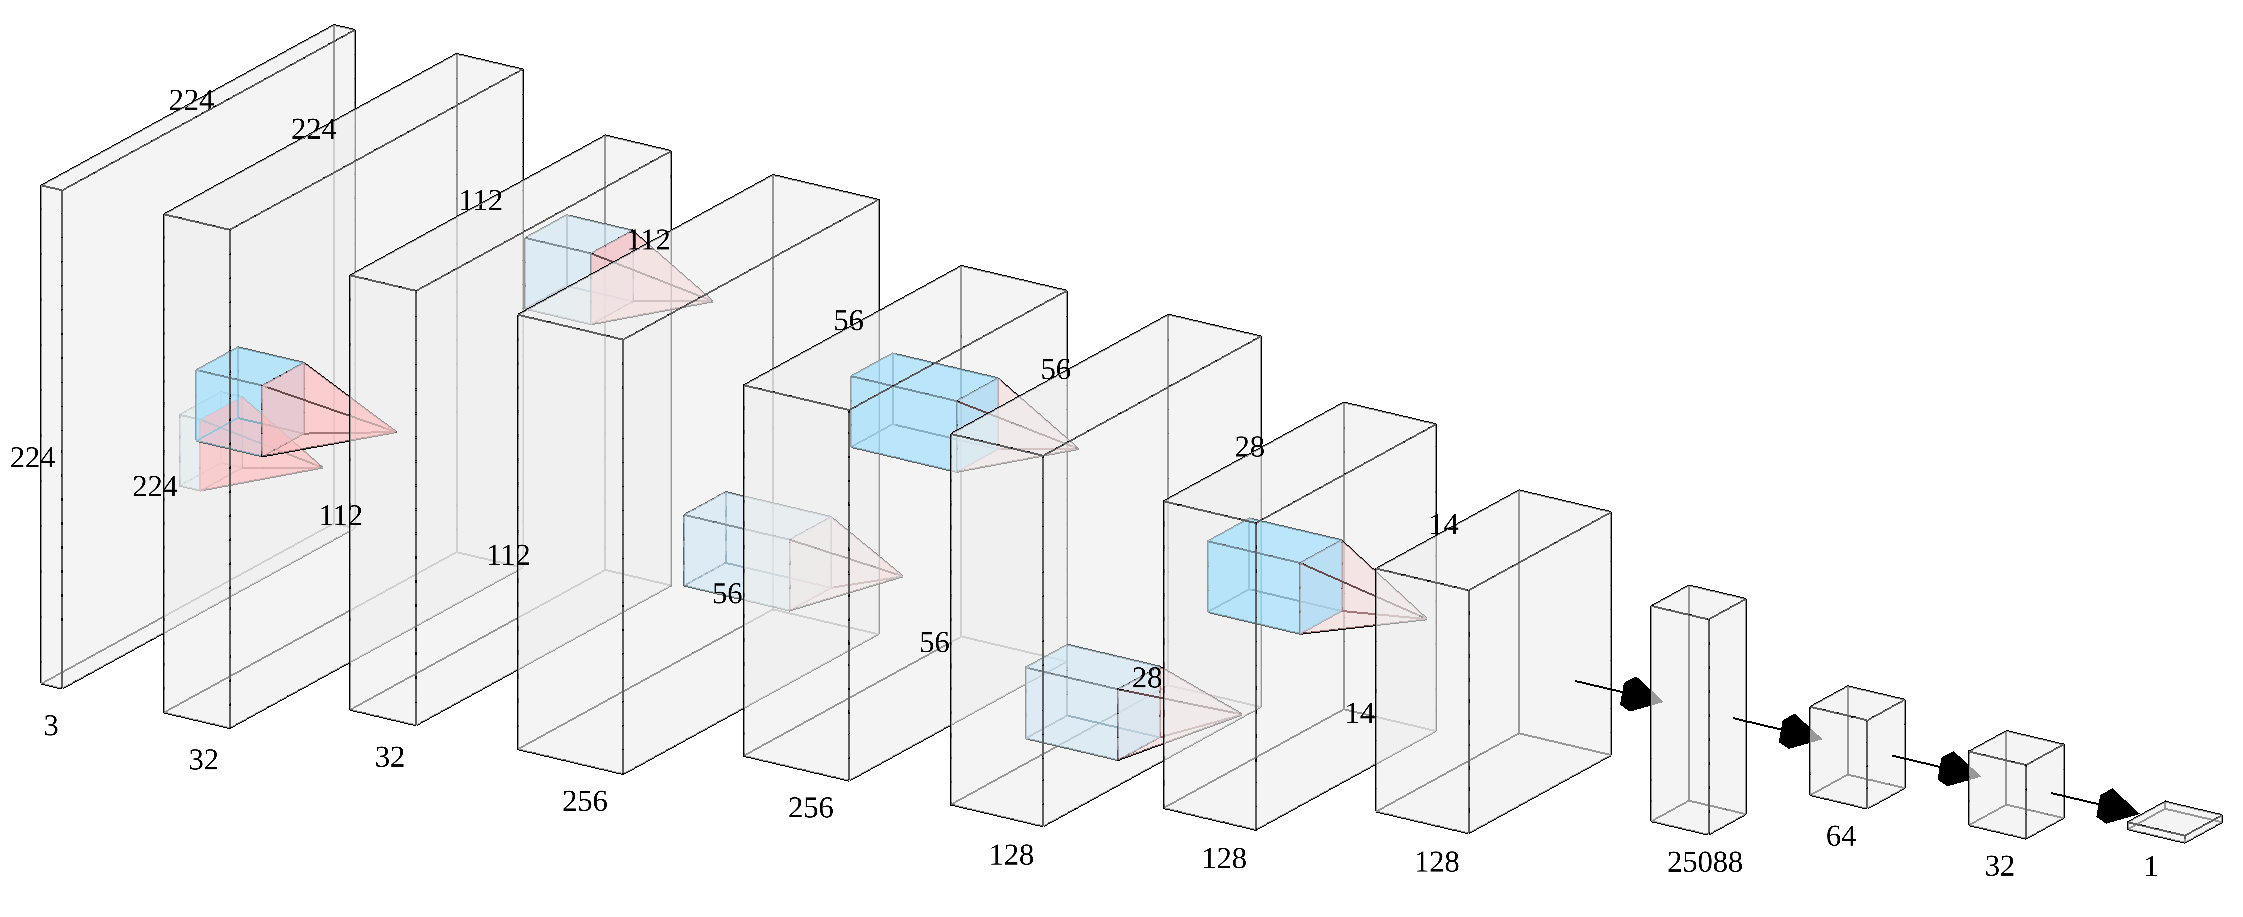
\includegraphics[scale=0.15]{/home/jacopo/PycharmProjects/muffin-stat-project/report/imgs/5_autotuned_netw_structure}
    \caption{
        Graphical representation of the autotuned CNN model structure\\
        \textit{Image generated via the NN-SVG tool}
    }
    \label{fig:5_autotuned_netw_structure}
\end{figure}
\begin{table}
    \centering
    \begin{tabular}{| c | c | c |}
        \hline
        $k$ & $accuracy$ & $l_{0-1}$ \\
        \hline\hline
        0   & 0.9248     & 0.0752    \\
        \hline
        1   & 0.9316     & 0.0684    \\
        \hline
        2   & 0.9524     & 0.0676    \\
        \hline
        3   & 0.9265     & 0.0735    \\
        \hline
        4   & 0.9205     & 0.0795    \\
        \hline
        \hline
        avg & 0.9272     & 0.0728    \\
        \hline
    \end{tabular}
    \caption{
        Left the first model's  \textit{k-fold-CV} estimates, middle second,  right the thrid one.
    }

    \label{tab:kfoldbestcnn}
\end{table}
